\documentclass[12pt,a4paper]{report}
\usepackage{graphicx}
\usepackage{amsmath}
\usepackage{fancyhdr}
\usepackage{cite}
\usepackage{framed}
\usepackage{a4wide}
\usepackage{float}
\usepackage{epsfig}
\usepackage{longtable}
\usepackage{enumerate}
\usepackage{afterpage}
\usepackage{multirow}
\usepackage{ragged2e}
\usepackage{gensymb}
\usepackage{amsfonts} 
\usepackage[left=3.5cm,top=1.5cm,right=3cm,bottom=4cm]{geometry}
\usepackage{setspace}           
\usepackage{float}
\usepackage{txfonts}
\usepackage{lipsum}

\newcommand{\Usefont}[1]{\fontfamily{#1}\selectfont}

\usepackage{lscape} % for landscape tables
\renewcommand{\baselinestretch}{1.7} 

\usepackage{blindtext}
\usepackage{xpatch}
\usepackage{url}
\usepackage{leqno}
\usepackage{subcaption}

\linespread{1.5}
\usepackage[intoc, english]{nomencl}
\hyphenpenalty=5000
\tolerance=1000
\usepackage[nottoc]{tocbibind}
\bibliographystyle{IEEEtran}
\renewcommand{\bibname}{References}

%*******************************************************************
%                        Header and Footer   
% This is not required in Technical reports submitted to CET ECE department.
% Please leave it commented                       
%*******************************************************************
%\pagestyle{fancy}
%\fancyhead{}
%\header and footer section
%\renewcommand\headrulewidth{0.1pt}
%\fancyhead[L]{\footnotesize \leftmark}
%\fancyhead[R]{\footnotesize \thepage}
%\renewcommand\headrulewidth{0pt}
%\fancyfoot[R]{\small College of Engineering Trivandrum}
%\renewcommand\footrulewidth{0.1pt}
%\fancyfoot[C]{2020 - 2021}
%\fancyfoot[L]{\small Title of the Seminar/Project}
%*******************************************************************


%*********************Figures*****************************
% Save all figures in the folder figures and include them in your 
% report using the command \includegraphics{figure-name}

\graphicspath{{figures/}}

% figure files can be in jpeg,jpg, png or pdf formats
%*******************************************************************


\begin{document}
	
	
%****The entries in this section are to be filled in by the student with appropriate values *************

% These values are used thoroughout the report 
% please fill in the appropriate values in the brackets {}

\gdef \title{TITLE OF PROJECT } % Project title
%\gdef \author{Student Name}	 %student name
\gdef \dept{Computer Science and Engineering} %Department
\gdef \degree{Bachelor of Technology} %degree
\gdef \branch{Computer Science and Engineering} %branch
\gdef \college{Government Engineering College, Thrissur} % Name of the College
\gdef \collegeplace{Thrissur} % Location of the College
\gdef \studentA{batch member 1} %Project batch member 1
\gdef \studentAroll{Register  no} % Project batch member 1 ktu id
\gdef \studentB{batch member 2} %Project batch member 2
\gdef \studentBroll{Register no} % Project batch member 2 ktu id

\gdef \studentC{batch member 3} %Project batch member 3
\gdef \studentCroll{Register no} % Project batch member 3 ktu id

\gdef \studentD{batch member 4} %Project batch member 4
\gdef \studentDroll{Register no} % Project batch member 4 ktu id

\gdef \guide{Project guide} %Project guide
\gdef \guidedes{Designation}%project guide designation

\gdef \guideco{Project co-guide} %Project coguide
\gdef \guidecodes{Designation}%project coguide designation

\gdef \guideext{ Project external guide} %Project external organisation guide
\gdef \guideextdes{Engineer/Scientist}%project external guide designation
\gdef \guideextorg{External guide organization} % Project external guide organization

\gdef \projcordinatorA{ Project Coordinator}% Project coordinator 1 
\gdef \projcordinatorAdes{Designation}% Project coordinator 1 designation

\gdef \projcordinatorB{ Project Coordinator 2} % Project coordinator 2 
\gdef \projcordinatorBdes{Designation}% Seminar coordinator 2 designation

\gdef \hod{ Head of the Department} %Head of Department
\gdef \hoddes{Designation} %HOD designation

\gdef \acadyear{2022 - 23} % Academic year
\gdef \month{JUNE 2023} %Month of Report submission
\gdef \date{15-06-2023} %Date of signing the declaration

%*******************************************************************
% The font pages. The source tex files are there in the folder
%==================================coverpage.tex================================


\newenvironment{coverpage}
\thispagestyle{empty}
\begin{titlepage}
	\begin{center}
		{\Usefont{phv} \Large \bf \title \par}
		\vspace*{40pt}
		\large \em \Usefont{pzc}{ 
			A Project Report \par
			submitted to the APJ Abdul Kalam Technological University\\
			in partial fulfillment of the requirements for the award of degree}\\ [.15\baselineskip] \par
		\Usefont{ppl} {\bfseries  \degree}\\
		in\\
		{\Usefont{ppl} {\bfseries \branch}}\\
		by\\
		\bf {\studentA}(\studentAroll)\\
		\bf {\studentB}(\studentBroll)\\
		\bf {\studentC}(\studentCroll)\\
		\bf {\studentD}(\studentDroll)\\
		\vspace*{40pt}
		\centering
		\begin{figure}[h!]
			\centerline{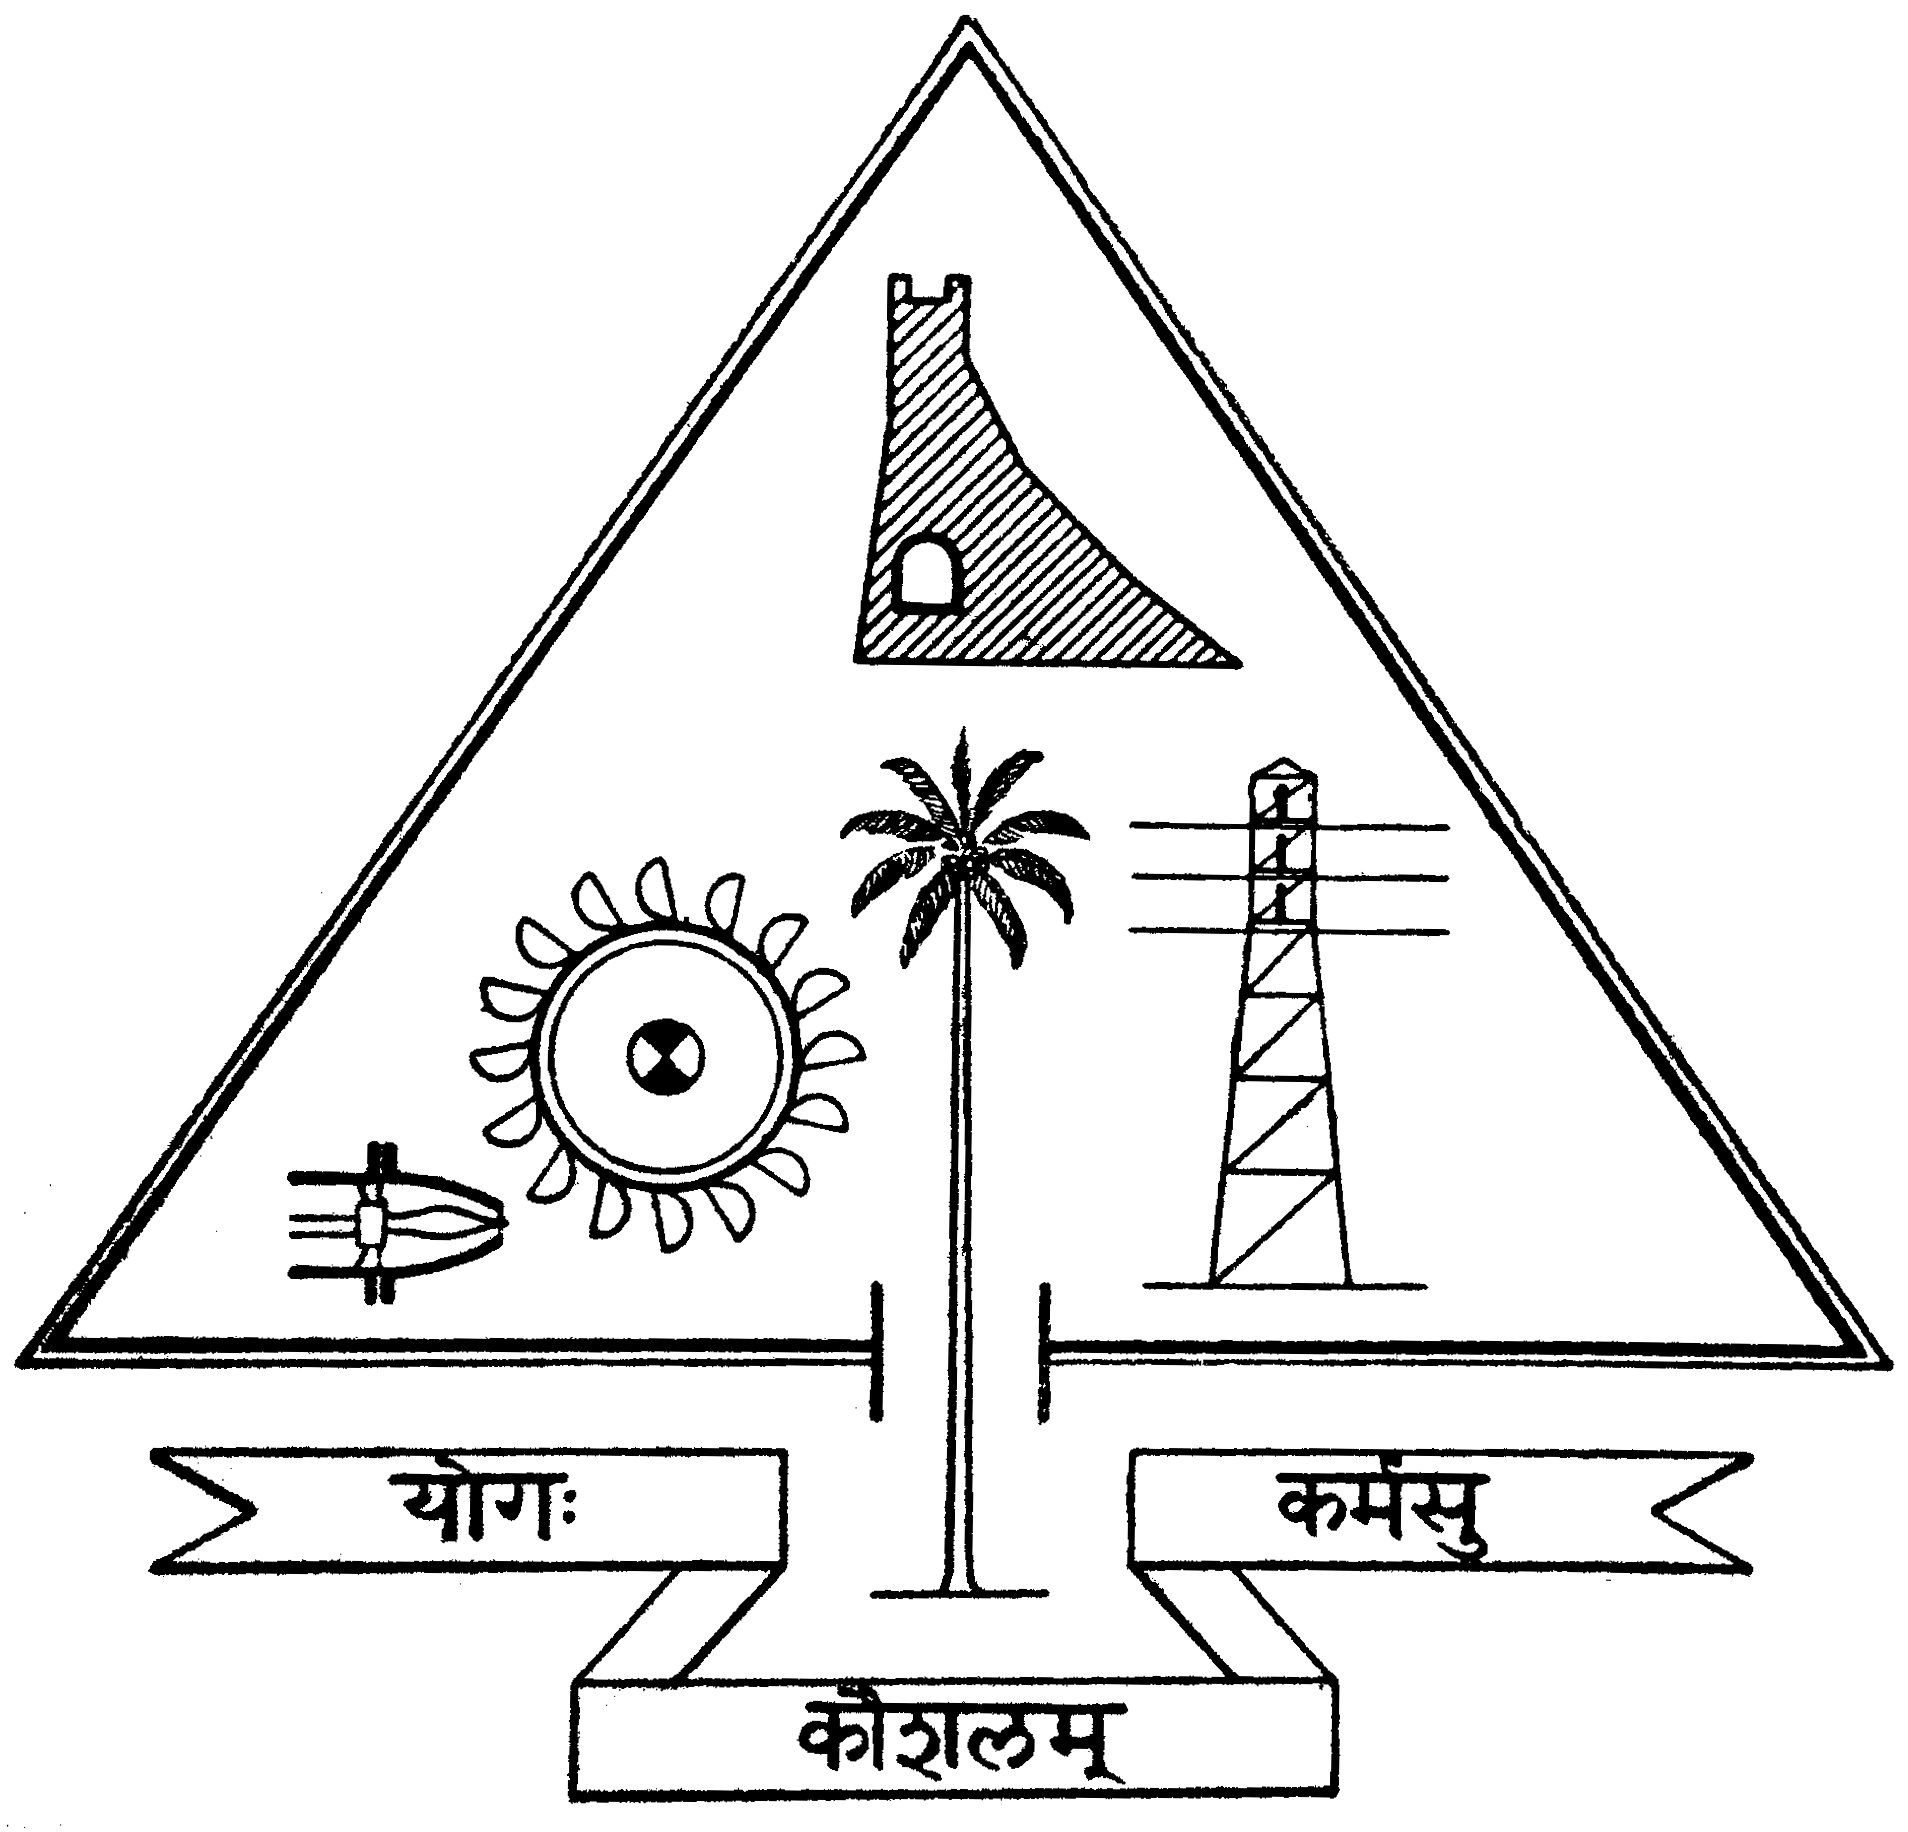
\includegraphics[scale=0.6]{gectemblem.jpg}}
		\end{figure}
		
		\vspace{\stretch{0.5}}
		\footnotesize{\bf DEPARTMENT OF COMPUTER SCIENCE AND ENGINEERING} \par
		\bf{GOVERNMENT ENGINEERING COLLEGE, THRISSUR} \par
		\bf{KERALA} \par
		\bf{\month}
	\end{center}		
\end{titlepage}	
 %Unless essential Do not edit this tex file



%%********************Certificate*******************

% To print name of only the project coordinator 1 in the certificate page
%==================================certificate1.tex================================
% To print name of only the seminar coordinator 1 in the certificate page

\newenvironment{certificate1}

	\newpage
	\begin{center}	
		%\vspace{1.5cm}
		
		\textbf{DEPARTMENT OF COMPUTER SCIENCE \& ENGINEERING\\}	
		\textbf{GOVERNMENT ENGINEERING COLLEGE\\}	
		\textbf{THRISSUR - 680009}
		
		 
	\end{center}
	
	\begin{center}
		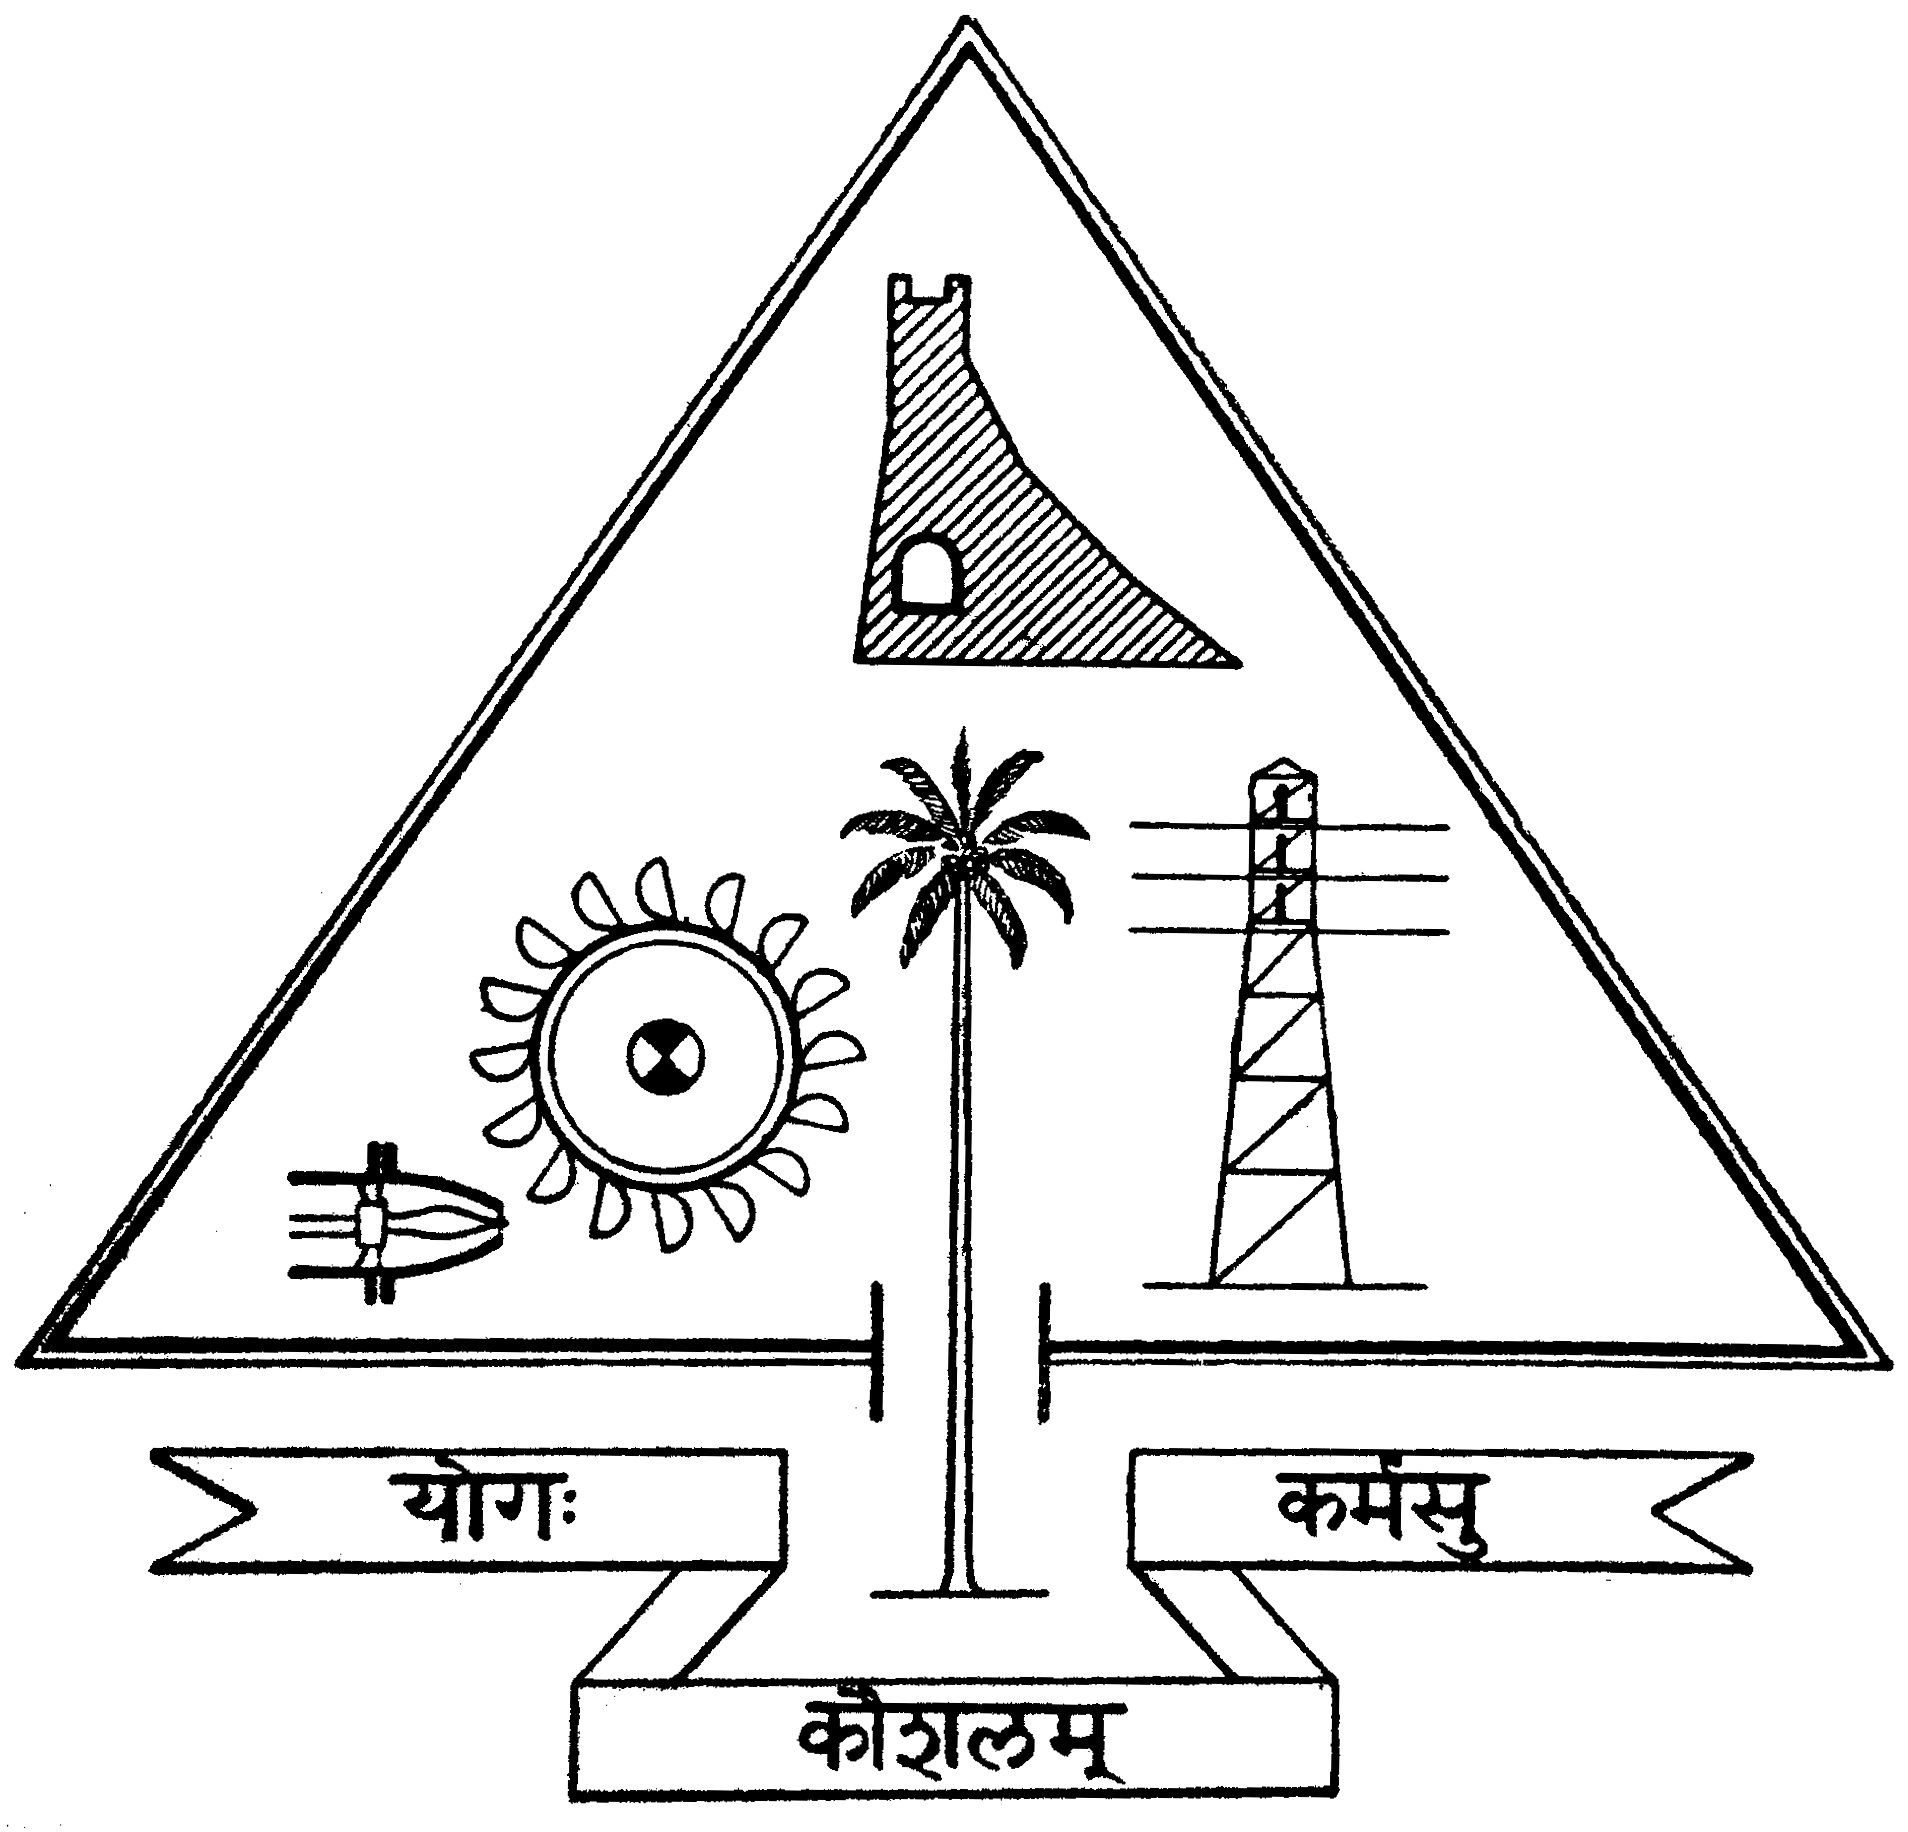
\includegraphics[scale=0.5]{gectemblem.jpg}	
	\end{center}
	\begin{center}
		\textbf{CERTIFICATE}
	\end{center}
	
	This is to certify that the report entitled \textbf{\title} submitted by \textbf{\studentA}\hspace*{2pt}(\studentAroll),\hspace*{2pt}\textbf{\studentB}\hspace*{2pt}(\studentBroll),\hspace*{2pt}\textbf{\studentC}\hspace*{2pt}(\studentCroll) \& \textbf{\studentD}\hspace*{2pt}(\studentDroll) to the APJ Abdul Kalam Technological University in partial fulfillment of the B.Tech.\ degree in \branch \hspace*{2pt} is a bonafide record of the project work carried out by him/her under our guidance and supervision. This report in any form has not been submitted to any other University or Institute for any purpose.
	
	
	\begin{singlespace}
		\vspace*{2cm}
		\begin{table}[h!]
			\centering
			\begin{tabular}{p{7cm} p{0.9cm} p{7cm}} 
				\textbf{\guide} && \textbf{\projcordinatorA} \\
				(Project Guide) &&  (Project Coordinator)\\
				\guidedes & & \projcordinatorAdes\\ 
				Department of CSE && Department of CSE\\ 
				GEC Thrissur & &GEC Thrissur\\
				
			\end{tabular}
			
		\end{table}
		
		\vspace*{1.3cm}
		
		\begin{center}
			
			%\hline
			\textbf{\hod} \\ 
			\hoddes\\ 
			Department of CSE\\ 
			GEC Thrissur\\
			Thrissur\\
			
		\end{center}
	\end{singlespace}
	
	\thispagestyle{empty}



 

% To print names of both the project coordinators in the certificate page
%%==================================certificate2.tex================================
% To print names of both the seminar coordinators in the certificate page
\newenvironment{certificate2}

\newpage
\begin{center}	
	%\vspace{1.5cm}
	
	\textbf{DEPT. OF ELECTRONICS \& COMMUNICATION ENGINEERING}	
	\textbf{COLLEGE OF ENGINEERING}	
	\textbf{TRIVANDRUM}
	
	\textbf{\acadyear} 
\end{center}

\begin{center}
	\includegraphics[scale=0.5]{cet_logo}	
\end{center}
\begin{center}
	\textbf{CERTIFICATE}
\end{center}

This is to certify that the report entitled \textbf{\title} submitted by \textbf{\author} \hspace*{2pt}(\rollno), to the APJ Abdul Kalam Technological University in partial fulfillment of the B.Tech.\ degree in \branch \hspace*{2pt} is a bonafide record of the seminar work carried out by him under our guidance and supervision. This report in any form has not been submitted to any other University or Institute for any purpose.


\begin{singlespace}
	\vspace*{2cm}
	\begin{table}[h!]
		\centering
		\begin{tabular}{p{7cm} p{0.9cm} p{7cm}} 
			\textbf{\guide} && \textbf{\semcordinatorA} \\
			(Seminar Guide) &&  (Seminar Coordinator)\\
			\guidedes & & \semcordinatorAdes\\ 
			\deptabbr && \deptabbr\\ 
			\college & &\college\\
			\collegeplace && \collegeplace\\
		\end{tabular}
		
	\end{table}
	
	\vspace*{1.3cm}
	
	\begin{center}
		\begin{tabular}{p{7cm} p{0.9cm} p{7cm}} 
			%\hline
			\textbf{\semcordinatorB} && \textbf{\hod} \\
			\semcordinatorBdes & & \hoddes\\ 
			\deptabbr && \deptabbr\\ 
			\college & &\college\\
			\collegeplace && \collegeplace\\
		\end{tabular}
	\end{center}
\end{singlespace}

\thispagestyle{empty}



 %Please uncomment this and comment the previous line

%%***************************************************


%==================================declaration.tex================================
%
\newpage
\newenvironment{declaration}
\thispagestyle{empty}
\begin{center}
\vspace*{50pt}
\textbf{DECLARATION}\\
\end{center}
We hereby declare that the project report {\bf{\title}}, submitted for partial fulfillment of the requirements for the award of degree of Bachelor of Technology of the APJ Abdul Kalam Technological University, Kerala is a bonafide work done by us under supervision of \textbf{Name of guide}.\par
This submission represents our ideas in our own words and where ideas or words of others have been included, we have adequately and accurately cited and referenced the original sources.\par 
We also declare that I have adhered to ethics of academic honesty and integrity and have not misrepresented or fabricated any data or idea or fact or source in our submission. We understand that any violation of the above will be a cause for disciplinary action by the institute and/or the
University and can also evoke penal action from the sources which have thus not been properly cited or from whom proper permission has not been obtained. This report has not been previously formed the basis for the award of any degree, diploma or similar title of any other University.

\noindent \begin{minipage}{0.45\linewidth}
\begin{flushleft}
\vspace{2.5cm}

\collegeplace \\
May 15, 2023

\end{flushleft} 
\end{minipage}
\hfill
\begin{minipage}{0.45\linewidth}
\begin{flushright}                                      
\vspace{1.5cm}

\textbf{\studentA}\\
\textbf{\studentB}\\
\textbf{\studentC}\\
\textbf{\studentD}\\


\end{flushright} 
\end{minipage}
\thispagestyle{empty}
 %Unless essential Do not edit this tex file

\pagenumbering{roman} 

%%********************************Abstract***********************
%============================= abstract.tex================================
\chapter*{Abstract}%
%\addcontentsline{toc}{chapter}{\numberline{}Abstract}%
\addcontentsline{toc}{chapter}{Abstract}%

\par This chapter should contain a brief of entire project. The abstract includes ideas leading to topic of project, explanation of project idea , what are the techniques used , results and future scope . The explanation cannot be vague keep it very short and precise.

\par Try to include all these within one page.
%\begin{flushright}
%	\textit{}
%\end{flushright}

\thispagestyle{plain}
%=======================================================================

 % Please type in the abstract in this tex file abstract.tex

%%***************************************************
% Default Acknowledgement page
%==================================acknowledgement.tex=============================
\chapter*{Acknowledgement}%
\addcontentsline{toc}{chapter}{Acknowledgement}%

%\newenvironment{acknowledgement}


\par We take this opportunity to express my deepest sense of gratitude and sincere thanks to everyone who helped us to complete this work successfully. We express our sincere thanks to \textbf{Name of HOD}, Head of Department, \dept, \college\hspace*{2pt} for providing  us with all the necessary facilities and support.\par

We would like to express my sincere gratitude to the \textbf{Name of project coordinators}, Designation, \hspace*{2pt} Department of \hspace*{2pt} \dept, \hspace*{2pt} \college \hspace*{2pt} \hspace*{2pt} for the support and co-operation.

We would like to place on record my sincere gratitude to our project guide \textbf{Name of project guide},\hspace*{2pt}\guidedes, \hspace*{2pt}\dept, \hspace*{2pt}\college \hspace*{2pt} %and our external guide \guideext,\hspace*{2pt}\guideextdes, \hspace*{2pt} \guideextorg   
for the guidance and mentorship throughout this work.

Finally I thank my family, and friends who contributed to the successful fulfilment of this project work.

\vspace*{30pt}
\begin{flushright}
	\textbf{\studentA}\\
	\textbf{\studentB}\\
	\textbf{\studentC}\\
	\textbf{\studentD}\\
\end{flushright}
\thispagestyle{plain}
  %Unless essential Do not edit this tex file


%%***************************************************
%%**If you have only one seminar coordinator faculty member
% please comment the above line and uncomment this line

%%==================================acknowledgement.tex=============================
\chapter*{Acknowledgement}%
\addcontentsline{toc}{chapter}{Acknowledgement}%

%\newenvironment{acknowledgement}


I take this opportunity to express my deepest sense of gratitude and sincere thanks to everyone who helped me to complete this work successfully. I express my sincere thanks to \textbf{ \hod}, Head of Department, \dept, \college\hspace*{2pt} \collegeplace \hspace*{2pt} for providing  me with all the necessary facilities and support.\par

 I would like to express my sincere gratitude to \textbf{\semcordinatorA}, \hspace*{2pt} department of \hspace*{2pt} \dept, \hspace*{2pt} \college \hspace*{2pt} \collegeplace \hspace*{2pt} for their support and co-operation.

\noindent I would like to place on record my sincere gratitude to my seminar guide \textbf{\guide},\hspace*{2pt}\guidedes,\hspace*{2pt}\dept,\hspace*{2pt}\college \hspace*{2pt} for the guidance and mentorship throughout the course.

Finally I thank my family, and friends who contributed to the succesful fulfilment of this seminar work.

\vspace*{30pt}
\begin{flushright}
	\textbf{\author}
\end{flushright}
\thispagestyle{plain}
  %Unless essential Do not edit this tex file
%*******************************************************************

\thispagestyle{empty}
\newpage
    
%%**********************Table of Contents***********************
\tableofcontents
\listoffigures
\listoftables
%==================================symbols.tex================================
% List of Symbols
\chapter*{ABBREVIATIONS}
\addcontentsline{toc}{chapter}{ABBREVIATIONS}%
%\makeatletter
%
%\makeatother
%%\newcommand{\abbrlabel}[1]{\makebox[3cm][l]{\textbf{#1}\ \tocfill}}
\begin{tabular}{l{1cm}l{5cm}} 
  \textbf{CNN} & Convolutional Neural Network \\ 
  \textbf{ML}& Machine Learning \\ 
  \textbf{IP} & Internet Protocol \\ 
\end{tabular}	





%==================================symbols.tex================================
% List of Symbols
\chapter*{List of Symbols}
\addcontentsline{toc}{chapter}{List of Symbols}%
%\makeatletter
%
%\makeatother
%%\newcommand{\abbrlabel}[1]{\makebox[3cm][l]{\textbf{#1}\ \tocfill}}

\newenvironment{symbols}

		
\begin{itemize}	\setlength{\itemsep}{0pt}
	\item [$\Omega$] \text{Unit of Resistance}
	\item[$\varepsilon^{'}$]  Real part of dielectric constant 
	\item[$\mbox{c}$]	Speed of light
	\item[$\lambda$]	Wavelength
	\item[$\delta$] Delta
\end{itemize}
		
%\begin{symbols}
%	\item \symbol{$\Omega$} \text{Unit of Resistance}
	
%	\item \symbol{[$\mu$]} 	\text{Magnetic permeability}
%	\item[$\mu_0$]	Magnetic permeability of free space
%	\item[$\varepsilon$] Relative complex dielectric constant
%	\item[$\varepsilon^{'}$]  Real part of dielectric constant 
%	\item[$\varepsilon^{''}$] Imaginary part of dielectric constant 
%	\item[$\varepsilon_{s}$] Snow surface dielectric constant
%	\item[$\mbox{c}$]	Speed of light
%	\item[$\lambda$]	Wavelength
%	\item[$\tau$] Pulse length of SAR signal
%	\item[$\beta$]  Bandwidth of the SAR signal
%	\item[$\theta$ ] 	Orientation angle 
%	\item[$\theta_{i}$] 	Incidence or local incidence angle
%	\item[$\theta_{r}$]  Local refractive angle 
%	\item[$\delta A$]	Azimuth resolution of the SAR data
%	\item[$L$]    SAR antenna length
%	\item[$\mathbf{E}(\mathbf{r},t)$] Electric field vector
%	\item[$\mathbf{E_{pq}^s}$]	Scattered field vector
%	\item[$\rho(\mathbf{r}, t)$] Volume density of free charges
%	\item[$\mathbf{g}_\mathbf{E}$] Stokes vector



%List of Symbols (Optional) comment if not required.
% symbold may be added in the file symbol.tex

%%********************Body of the report**********
% Arabic numbering is used in the body of the report

\cleardoublepage
\setcounter{page}{1}
\pagenumbering{arabic}

%%********************Chapter 1**********
\chapter{Introduction}
%\lipsum[1] % Please comment this line and type in the introduction chapter
\section{Topic Introduction}
Explain what motivates to the topic of project. Give an introduction to area , problems existing to be solved  etc. 
\section{Problem Statement}
Issues existing in the particular area you have chosen should identified and stated here. Also clearly and precisely state the \textbf{PROBLEM TO BE SOLVED THROUGH PROJECT IMPLEMENTATION}.
\section{Objectives}
The aims of project to be implemented . List the objectives to be solved through the implementation of your project.
\section{Novelty of Idea and Implementation Steps}
\section{Societal and Industrial Relevance }
How the project will be useful in solving a problem which is relevant to the paarticular industry as well as how it will be helpful to the societal people around you.
%%********************Chapter 2**********
\chapter{Literature Review}
\section{Topic of review-Section Wise Review}
\subsection{Subtopics if any}
Add subsections as you studied and done review. Change the subsection headings according to your review.
\section{Conclusions and Gap Analysis}
Conclusions can be stated as subsections as done in previous section or as an overall conclusion. Also include gap analysis which refers to the non existing solutions in the area which may lead you to the solution proposed.
\section{Summary}
Explain how project title and objectives influenced by review.

Reference \cite{india}, \cite{rpi}, . See figure \ref{net2} .

\begin{figure}[h!]
	\centering
	\includegraphics[width=0.9\linewidth]{ospf}
	\caption{Autonomous System Hierarchy}
	\label{net2}
\end{figure}


\noindent The system is described by the equation \ref{sys_eq1} below. 

\begin{equation} \label{sys_eq1}
y = mx + c
\end{equation}




%%********************Chapter 3**********
\chapter{Feasibility Study and Requirements Analysis}


\section{Feasibility}
%\lipsum[2] % Please comment this line and type in the content


\subsection{Technical Feasibility}
Should include feasibility studies in terms of software ,  data , hardware.
\subsection{Economic Feasibility}
\subsection{Time Feasibility}
\subsection{Legal Feasibility}
\subsection{Operational Feasibility}
\section{Project Requirements}
Explain the SRS of the project. The explanation should be done as in following subsections
\subsection{Implementation Requirements}
Do not state the requirements you used  but include minimum requirements for the implementation of your proposed solution.
\subsection{Deployment Requirements}
%\lipsum[3] % Please comment this line and type in the content

%%********************Chapter 4**********
\chapter{Project Design}
Use your SDD done previously.
\chapter{Implementation and Testing}
You are not expected to list software or tools used. You should explain how each were used in the project for each sections.
Demonstrate the transformation of input to output with your processes involved ie, how your process changes input to output. First state the expected outputs .
List some test cases with test outputs.
\chapter{Results and Discussion}
% Please comment this line and type in the content

Showcase your obtained results with a discussion between expected and testing outputs. You should state that to which extend you have achieved your goal. 
 % Please comment this line and type in the content
\begin{table}[h!]
	\centering
	\caption{test table}
	\vspace*{5pt}
	\begin{tabular}{|c|c|c|}
		\hline
		Sl. No & Item 1 & Itm 2 \\ \hline
		1      & 37     & 45    \\ \hline
		2      & 42     & 23    \\ \hline
		3      & 47     & 1     \\ \hline
		4      & 52     & -21   \\ \hline
		5      & 57     & -43   \\ \hline
		6      & 62     & -65   \\ \hline
		7      & 67     & -87   \\ \hline
		8      & 72     & -109  \\ \hline
		9      & 77     & -131  \\ \hline
		10     & 82     & -153  \\ \hline
	\end{tabular}
\end{table}

%%********************Chapter 5**********
\chapter{Conclusions and Future Scope}

%\lipsum[2] 

%%********************References**********
%%****This template uses IEEE bibliography style

 \begin{thebibliography}{99}
	\bibitem{india} HU, Yun Chao, et al., \emph{Mobile edge computing?A key technology
		towards 5G}, ETSI white paper, 2015, vol. 11, no 11, p. 1-16.
	
	
	\bibitem{rpi}
	@online{ Raspberry pi,
		\url{https://www.raspberrypi.org/}
		Online; accessed 10-June-2019
	}
	
	\bibitem{japan} HU, Yun Chao, et al., \emph{Mobile edge computing?A key technology
		towards 5G}, ETSI white paper, 2015, vol. 11, no 11, p. 1-16.		
\end{thebibliography}

\end{document}